\documentclass[notes,11pt, aspectratio=169]{beamer}

\usepackage{pgfpages}
% These slides also contain speaker notes. You can print just the slides,
% just the notes, or both, depending on the setting below. Comment out the want
% you want.
\setbeameroption{hide notes} % Only slide
%\setbeameroption{show only notes} % Only notes
%\setbeameroption{show notes on second screen=right} % Both
\setbeamertemplate{caption}{\raggedright\insertcaption\par}


\usepackage{helvet}
\usepackage[default]{lato}
\usepackage{array}

\usepackage[backend=biber,style=authoryear,
sorting=ynt,citestyle=authoryear]{biblatex}
\addbibresource{Paper/papercitations.bib}

\usepackage{tikz}
\usepackage{verbatim}
\setbeamertemplate{note page}{\pagecolor{yellow!5}\insertnote}
\usetikzlibrary{positioning}
\usetikzlibrary{snakes}
\usetikzlibrary{calc}
\usetikzlibrary{arrows}
\usetikzlibrary{decorations.markings}
\usetikzlibrary{shapes.misc}
\usetikzlibrary{matrix,shapes,arrows,fit,tikzmark}
\usepackage{amsmath}
\usepackage{mathpazo}
\usepackage{hyperref}
\usepackage{lipsum}
\usepackage{multimedia}
\usepackage{graphicx}
\usepackage{multirow}
\usepackage{graphicx}
\usepackage{dcolumn}
\usepackage{bbm}
\newcolumntype{d}[0]{D{.}{.}{5}}
\usepackage{subfigure}
\usepackage{import}
\usepackage{fontawesome5}

\usepackage[backend=biber,style=authoryear,
sorting=nyt,citestyle=authoryear]{biblatex}
\addbibresource{papercitations.bib}

\usepackage{changepage}
\usepackage{appendixnumberbeamer}
\newcommand{\beginbackup}{
   \newcounter{framenumbervorappendix}
   \setcounter{framenumbervorappendix}{\value{framenumber}}
   \setbeamertemplate{footline}
   {
     \leavevmode%
     \hline
     box{%
       \begin{beamercolorbox}[wd=\paperwidth,ht=2.25ex,dp=1ex,right]{footlinecolor}%
%         \insertframenumber  \hspace*{2ex} 
       \end{beamercolorbox}}%
     \vskip0pt%
   }
 }
\newcommand{\backupend}{
   \addtocounter{framenumbervorappendix}{-\value{framenumber}}
   \addtocounter{framenumber}{\value{framenumbervorappendix}} 
}

\setbeamertemplate{blocks}[rounded]
\setbeamercolor{block title}{bg=eggplant!70, fg=white}
\setbeamercolor{block body}{bg=eggplant!30}

\usepackage{graphicx}
\usepackage[space]{grffile}
\usepackage{booktabs}

% These are my colors -- there are many like them, but these ones are mine.
\definecolor{sage}{RGB}{102,153,102}
\definecolor{cambridgeblue}{RGB}{104, 166, 145}
\definecolor{yellow}{RGB}{255,173,1}
\definecolor{purple}{RGB}{153,102,153}
\definecolor{ashgray}{RGB}{191, 211, 193}
\definecolor{eggplant}{RGB}{105, 79, 93}
\definecolor{silver}{RGB}{192, 197, 193}
\definecolor{darkcyan}{RGB}{78, 135, 140}
\definecolor{lightcyan}{RGB}{201, 228, 231}
\definecolor{columbiablue}{RGB}{187, 213, 237}
\definecolor{lightblue}{RGB}{184, 219, 217}
\definecolor{earthyellow}{RGB}{234, 180, 100}

\setbeamercolor{mycolor}{fg=white,bg=sage}

% colors for diagrams
\definecolor{diagramtan}{RGB}{225,190,106}
\definecolor{diagramteal}{RGB}{64, 176, 166}
\definecolor{diagrampurple}{RGB}{170, 131, 239}
\definecolor{diagramred}{RGB}{146, 79, 79}


\hypersetup{
  colorlinks=false,
  linkbordercolor = {white},
  linkcolor = {sage}
}

\newcommand{\btVFill}{\vskip0pt plus 1filll}


%% I use a beige off white for my background
\definecolor{MyBackground}{RGB}{255,253,218}

%% Uncomment this if you want to change the background color to something else
%\setbeamercolor{background canvas}{bg=MyBackground}

%% Change the bg color to adjust your transition slide background color!
\newenvironment{transitionframe}{
  \setbeamercolor{background canvas}{bg=lightcyan}
  \begin{frame}[plain,noframenumbering]}{
    \end{frame}
}

\setbeamercolor{frametitle}{fg=black, bg=lightcyan}
\setbeamercolor{title}{fg=black}
\setbeamertemplate{footline}{%
  \raisebox{5pt}{\makebox[\paperwidth]{\hfill\makebox[15pt]{\scriptsize\insertframenumber}}}}
\setbeamertemplate{navigation symbols}{} 
\setbeamertemplate{itemize items}{$\bullet$}
\setbeamercolor{itemize item}{fg=lightcyan}
\setbeamercolor{itemize subitem}{fg=lightcyan}
\setbeamercolor{enumerate item}{fg=black}
\setbeamercolor{enumerate subitem}{fg=black}
\setbeamercolor{button}{bg=eggplant!80,fg=white}

\setbeamertemplate{frametitle}
{
    \nointerlineskip
    \begin{beamercolorbox}[sep=0.3cm,ht=2em,wd=\paperwidth]{frametitle}
        \vbox{}\vskip-2ex%
        \strut\insertframetitle\strut
        \vskip-0.8ex%
    \end{beamercolorbox}
}



% If you like road maps, rather than having clutter at the top, have a roadmap show up at the end of each section 
% (and after your introduction)
% Uncomment this is if you want the roadmap!
% \AtBeginSection[]
% {
%    \begin{frame}
%        \frametitle{Roadmap of Talk}
%        \tableofcontents[currentsection]
%    \end{frame}
% }

\setbeamercolor{section in toc}{fg=sage}
\setbeamercolor{subsection in toc}{fg=sage}
\setbeamersize{text margin left=1em,text margin right=1em} 

\newenvironment{wideitemize}{\itemize\addtolength{\itemsep}{10pt}}{\enditemize}

\usepackage{environ}
\NewEnviron{videoframe}[1]{
  \begin{frame}
    \vspace{-8pt}
    \begin{columns}[onlytextwidth, T] % align columns
      \begin{column}{.58\textwidth}
        \begin{minipage}[t][\textheight][t]
          {\dimexpr\textwidth}
          \vspace{8pt}
          \hspace{4pt} {\Large \sc \textcolor{blue}{#1}}
          \vspace{8pt}
          
          \BODY
        \end{minipage}
      \end{column}%
      \hfill%
      \begin{column}{.42\textwidth}
        \colorbox{green!20}{\begin{minipage}[t][1.2\textheight][t]
            {\dimexpr\textwidth}
            Face goes here
          \end{minipage}}
      \end{column}%
    \end{columns}
  \end{frame}
}

\title[]{\textcolor{sage}{Does Hospital Leadership Matter? \newline
Evidence from Pay-for-Performance}}

\author[]{Hanna Glenn}
\date{}


\begin{document}

%%% TIKZ STUFF
\tikzset{   
        every picture/.style={remember picture,baseline},
        every node/.style={anchor=base,align=center,outer sep=1.5pt},
        every path/.style={thick},
        }
\newcommand\marktopleft[1]{%
    \tikz[overlay,remember picture] 
        \node (marker-#1-a) at (-.3em,.3em) {};%
}
\newcommand\markbottomright[2]{%
    \tikz[overlay,remember picture] 
        \node (marker-#1-b) at (0em,0em) {};%
}
\tikzstyle{every picture}+=[remember picture] 
\tikzstyle{mybox} =[draw=black, very thick, rectangle, inner sep=10pt, inner ysep=20pt]
\tikzstyle{fancytitle} =[draw=black,fill=red, text=white]
%%%% END TIKZ STUFF

% Title Slide
\begin{frame}[plain]
% Background image
\begin{tikzpicture}[remember picture,overlay]
    \node
[
    above=0.5cm,
    align=center,
    fill=lightcyan,
    rounded corners,
    inner xsep=15pt,
    inner ysep=10pt, 
    minimum width=0.9\textwidth,
    text width=0.9\textwidth
] (title) at (current page.center)
{
    \LARGE Beyond Mergers: \\
    
    \vspace{3mm}
    \Large Informal Governance Ties and Hospital Behavior
};
% Author 
\node[below=1cm] (author) at (title.south){\large Hanna Glenn, The University of Queensland};
% Date
\node[below=0.25cm] (date) at (author.south){\today};
\end{tikzpicture}
    
\end{frame}

\section{Intro}

\large

\begin{frame}{Anti-trust Regulation}
    \begin{columns}
        \column{0.5\textwidth}
            \begin{figure}
                \centering
                \caption{Percent of HRRs with HHI $>$ 1,800}
                \includegraphics[width=\linewidth]{Objects/hhi_graph.pdf}
            \end{figure}

        \column{0.5\textwidth}
            \begin{wideitemize}
                \item Hospital markets are becoming increasingly concentrated
                \item 1,600 mergers from 1998 to 2017 \small (\cite{gaynor2020health}) \large
                \item This has led to increased scrutiny of mergers and acquisitions
            \end{wideitemize}
    \end{columns}
\end{frame}

\begin{frame}[t]{The Big Idea}
\centering

\vspace{15mm}

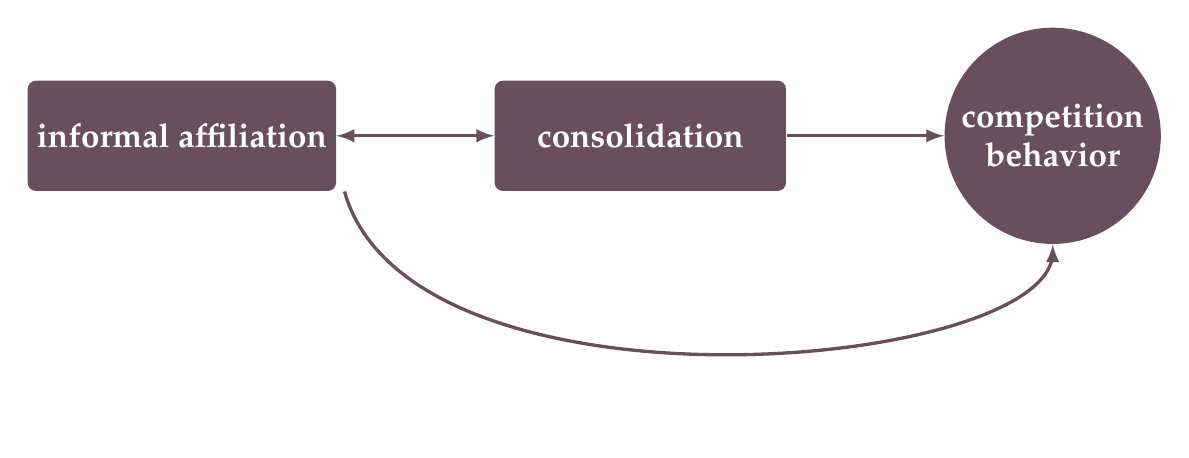
\begin{tikzpicture}[
    node distance=2cm,
    >=latex,
    % node styles
    box/.style = {
      draw=none,
      rounded corners=3pt,
      minimum width=3.7cm,
      minimum height=1.4cm,
      align=center,
      font=\bfseries\large,
      text=white
    },
    circ/.style = {
      circle,
      minimum size=2.4cm,
      align=center,
      font=\bfseries\large,
      text=white,
      draw=none
    },
    % arrow styles
    twoarr/.style = {<->, line width=1.2pt, draw=eggplant},
    arr/.style = {->, line width=1.2pt, draw=eggplant},
    underarr/.style= {->, line width=1.2pt, draw=eggplant}
  ]

  % --- Nodes
  \node[box, fill=eggplant] (affil) {informal affiliation};

  \node[box, fill=eggplant, right=of affil] (cons) {consolidation};

  \node[circ, fill=eggplant, right=of cons] (comp) {competition\\behavior};

  % --- Arrows
  \draw[twoarr] (affil) -- (cons);
  \draw[arr]  (cons) -- (comp);
    \path
    (affil.south east) ++(0.1cm,0) coordinate (startBelow);
  \path
    (comp.south) ++(0,-1.6cm) coordinate (midBelow); % how far down to dip
  \draw[underarr]
    (startBelow)
      .. controls ($(affil.south)!0.5!(cons.south) + (0,-3cm)$) and (midBelow) ..
    ($(comp.south) + (0,-0.1cm)$) -- (comp);
  

\end{tikzpicture}
\end{frame}

\section{Hospital Consolidation Intro}

\begin{frame}[t]{What We Already Know (Hospitals)}
\centering

\vspace{15mm}

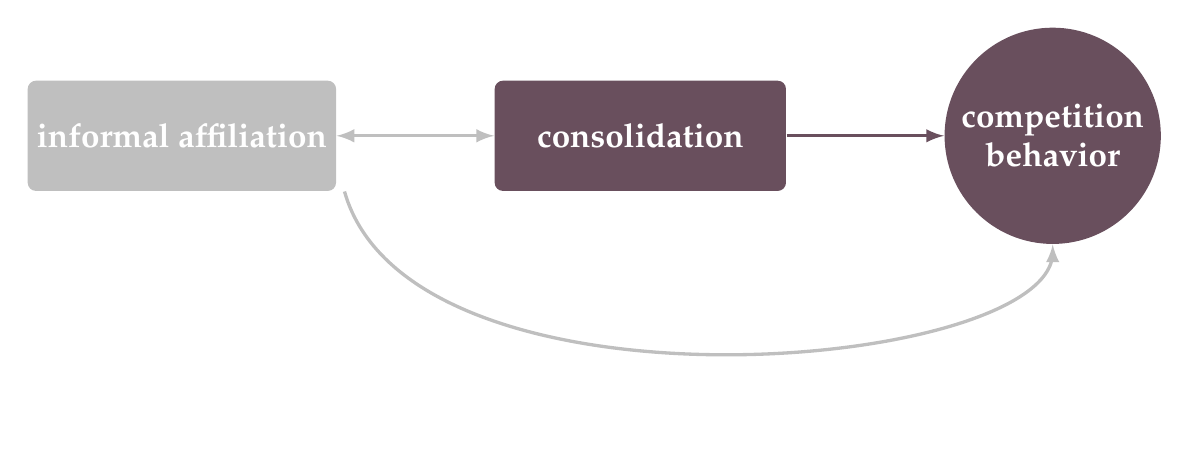
\begin{tikzpicture}[
    node distance=2cm,
    >=latex,
    % node styles
    box/.style = {
      draw=none,
      rounded corners=3pt,
      minimum width=3.7cm,
      minimum height=1.4cm,
      align=center,
      font=\bfseries\large,
      text=white
    },
    circ/.style = {
      circle,
      minimum size=2.4cm,
      align=center,
      font=\bfseries\large,
      text=white,
      draw=none
    },
    % arrow styles
    twoarr/.style = {<->, line width=1.2pt, draw=lightgray},
    arr/.style = {->, line width=1.2pt, draw=eggplant},
    underarr/.style= {->, line width=1.2pt, draw=lightgray}
  ]

  % --- Nodes
  \node[box, fill=lightgray] (affil) {informal affiliation};

  \node[box, fill=eggplant, right=of affil] (cons) {consolidation};

  \node[circ, fill=eggplant, right=of cons] (comp) {competition\\behavior};

  % --- Arrows
  \draw[twoarr] (affil) -- (cons);
  \draw[arr]  (cons) -- (comp);
    \path
    (affil.south east) ++(0.1cm,0) coordinate (startBelow);
  \path
    (comp.south) ++(0,-1.6cm) coordinate (midBelow); % how far down to dip
  \draw[underarr]
    (startBelow)
      .. controls ($(affil.south)!0.5!(cons.south) + (0,-3cm)$) and (midBelow) ..
    ($(comp.south) + (0,-0.1cm)$) -- (comp);
  

\end{tikzpicture}
\end{frame}


\begin{frame}{Hospital Consolidation Literature}
Operating costs/efficiency
\begin{itemize}
    \item Early studies found no effect \small (\cite{alexander1996short}; \cite{ho2000hospital}) \large
    \item More recent work does document increased efficiency \small (\cite{schmitt2017hospital}; \cite{andreyeva2024corporatization}; \cite{craig2021mergers}) \large
\end{itemize}

\vspace{1mm}

Price/quality
\begin{itemize}
    \item Consistently raised prices \small (\cite{gaynor2012impact}; \cite{boozary2019association}; \cite{cooper2019price}; \cite{andreyeva2024corporatization}) \large
    \item Very mixed evidence on quality \small (\cite{haas2011mergers}; \cite{beaulieu2020changes}; \cite{hayford2012impact}; \cite{andreyeva2024corporatization}) \large
\end{itemize}

\vspace{1mm}

Other behaviors/mechanisms
    \begin{itemize}
        \item Convergence in treatment styles \small (\cite{eliason2020acquisitions}) \large
        \item Changes in treatment styles \small (\cite{mariani2022impact}) \large
        \item Shifts in admission patterns \small (\cite{desai2023hospital}) \large
    \end{itemize}

    \vspace{2mm}

\textit{Effects are mitigated with more distance between the hospitals \small  (\cite{cooper2019price}) \large}

\end{frame}

\section{Informal Affiliation Intro}

\begin{frame}[t]{What We Know Less About}
\centering

\vspace{15mm}

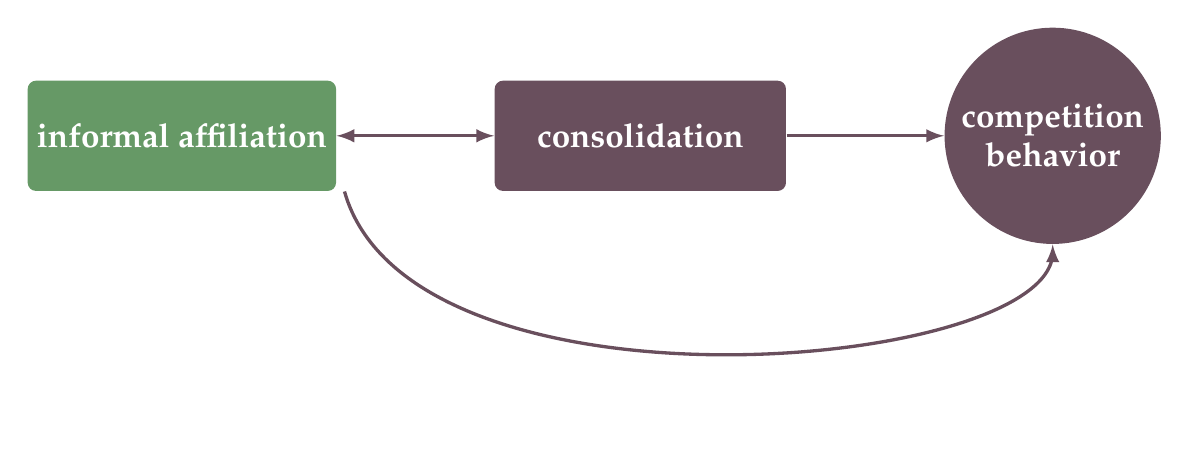
\begin{tikzpicture}[
    node distance=2cm,
    >=latex,
    % node styles
    box/.style = {
      draw=none,
      rounded corners=3pt,
      minimum width=3.7cm,
      minimum height=1.4cm,
      align=center,
      font=\bfseries\large,
      text=white
    },
    circ/.style = {
      circle,
      minimum size=2.4cm,
      align=center,
      font=\bfseries\large,
      text=white,
      draw=none
    },
    % arrow styles
    twoarr/.style = {<->, line width=1.2pt, draw=eggplant},
    arr/.style = {->, line width=1.2pt, draw=eggplant},
    underarr/.style= {->, line width=1.2pt, draw=eggplant}
  ]

  % --- Nodes
  \node[box, fill=sage] (affil) {informal affiliation};

  \node[box, fill=eggplant, right=of affil] (cons) {consolidation};

  \node[circ, fill=eggplant, right=of cons] (comp) {competition\\behavior};

  % --- Arrows
  \draw[twoarr] (affil) -- (cons);
  \draw[arr]  (cons) -- (comp);
    \path
    (affil.south east) ++(0.1cm,0) coordinate (startBelow);
  \path
    (comp.south) ++(0,-1.6cm) coordinate (midBelow); % how far down to dip
  \draw[underarr]
    (startBelow)
      .. controls ($(affil.south)!0.5!(cons.south) + (0,-3cm)$) and (midBelow) ..
    ($(comp.south) + (0,-0.1cm)$) -- (comp);
  

\end{tikzpicture}
\end{frame}

\begin{frame}{Unregulated Consolidation}
    While they don't commonly garner national attention, there are other hospital affiliations that could be important

    \vspace{10mm}

    \begin{columns}[T]
        \column{0.5\textwidth}
        \centering
        \textcolor{eggplant}{Small-scale Mergers}

        \vspace{3mm}

        \begin{wideitemize}
        \item ``Stealth mergers"
            \item Can reduce competition \\ \small (\cite{majerovitz2021consolidation}; \cite{aggarwal2025stealth}; \cite{wollmann2019stealth}; \cite{wollmann2020get}; \cite{kepler2023stealth}) \large
        \end{wideitemize}

        \column{0.5\textwidth}
        \centering
        \textcolor{eggplant}{Informal Affiliations}

        \vspace{3mm}

        \begin{wideitemize}
            \item Joint ventures; Clinical agreements; Shared members of leadership
            \item Several states have begun regulation these types of affiliations
        \end{wideitemize}
    \end{columns}
\end{frame}

\begin{frame}{Informal Affiliations: A Note of Transparency}
    In this paper, how I measure informal affiliation is strictly by \underline{overlapping leadership}

    \vspace{10mm}

    This is important and relevant on its own
    \begin{itemize}
        \item In the Clayton Act
        \item FTC has targeted it directly
    \end{itemize}

    \vspace{3mm}

    However, could be correlated with other types of affiliation
    \begin{itemize}
        \item There is no data to verify this
        \item I will investigate mechanisms to try to tease it out
    \end{itemize}

\end{frame}

\section{Overlapping Leaders}

\begin{frame}{Overlapping Leaders: Does it Actually Happen?}
    \begin{columns}[T]
        \column{0.4\linewidth}
        \centering
        \includegraphics[width=0.9\textwidth]{clips/sevita_news.png}

        \column{0.6\linewidth}
        \centering
        \includegraphics[width=0.9\textwidth]{clips/affiliation1.png}

        \vspace{3mm}
        \includegraphics[width=0.9\textwidth]{clips/affiliation2.png}
    \end{columns}
\end{frame}

\begin{frame}{Overlapping Leaders: Should it Actually Matter?}
    Board of Directors

    \vspace{2mm}
    \begin{wideitemize}
        \item Sets the broad direction of the firm and provides oversight
        \item Not in charge of day-to-day operations
    \end{wideitemize}

    \vspace{5mm}

    Board Governance is Correlated with Hospital Outcomes

    \vspace{2mm}
    \begin{wideitemize}
        \item Level of influence over the CEO \small (\cite{golden2001will}; \cite{alexander2008governance}; \cite{jiang2012enhancing}) \large
        \item Since the ACA, boards have been more directly involved in quality oversight \small (\cite{jha2010hospital}; \cite{prybil2010board}) \large
    \end{wideitemize}
\end{frame}

\begin{frame}[t]{This Paper}
\centering

\vspace{15mm}

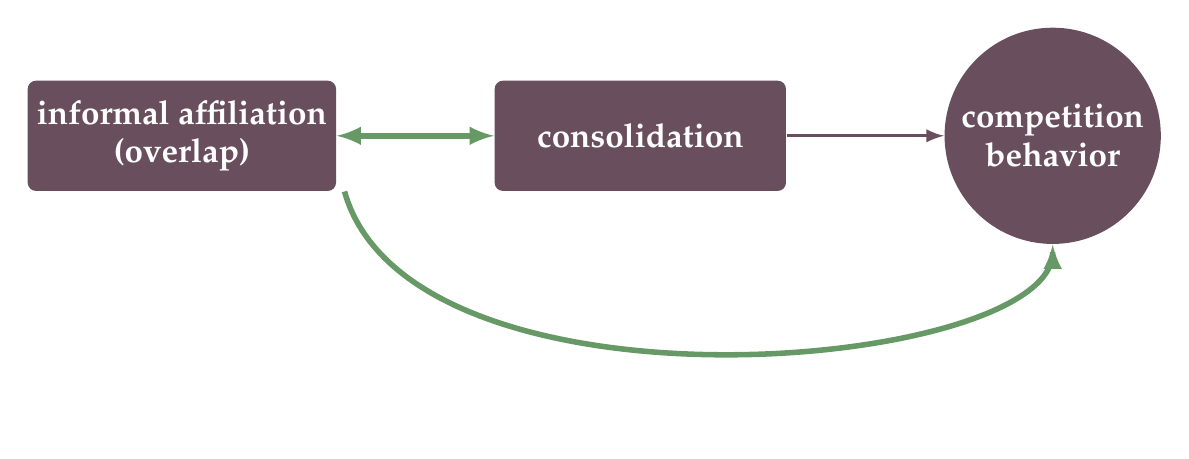
\begin{tikzpicture}[
    node distance=2cm,
    >=latex,
    % node styles
    box/.style = {
      draw=none,
      rounded corners=3pt,
      minimum width=3.7cm,
      minimum height=1.4cm,
      align=center,
      font=\bfseries\large,
      text=white
    },
    circ/.style = {
      circle,
      minimum size=2.4cm,
      align=center,
      font=\bfseries\large,
      text=white,
      draw=none
    },
    % arrow styles
    twoarr/.style = {<->, line width=2pt, draw=sage},
    arr/.style = {->, line width=1.2pt, draw=eggplant},
    underarr/.style= {->, line width=2pt, draw=sage}
  ]

  % --- Nodes
  \node[box, fill=eggplant] (affil) {informal affiliation\\(overlap)};

  \node[box, fill=eggplant, right=of affil] (cons) {consolidation};

  \node[circ, fill=eggplant, right=of cons] (comp) {competition\\behavior};

  % --- Arrows
  \draw[twoarr] (affil) -- (cons);
  \draw[arr]  (cons) -- (comp);
    \path
    (affil.south east) ++(0.1cm,0) coordinate (startBelow);
  \path
    (comp.south) ++(0,-1.6cm) coordinate (midBelow); % how far down to dip
  \draw[underarr]
    (startBelow)
      .. controls ($(affil.south)!0.5!(cons.south) + (0,-3cm)$) and (midBelow) ..
    ($(comp.south) + (0,-0.1cm)$) -- (comp);
  

\end{tikzpicture}
\end{frame}

\section{Data}

\begin{frame}{Data on Boards/Executives}
\begin{itemize}
    \item Tax Forms 990s: Nonprofits
    \item 2013-2023
\end{itemize}

\vspace{5mm}

\begin{table}[ht!]
\centering
\begin{tabular}[t]{lccccc}
\toprule
 & Num. People & Doctor & Nurse & Health Admin. & Female\\
\midrule
\addlinespace[0.3em]
Board Members & 32,678 & 0.18 & 0.03 & 0 & 0.30\\
Executives & 19,344 & 0.14 & 0.03 & 0 & 0.38\\
\bottomrule
\end{tabular}
\end{table}
\large
    
\end{frame}

\begin{frame}{Documenting Overlap}
    \begin{figure}
        \centering
        \caption{Prevalence of Board/Executive Overlap}
        \includegraphics[width=0.8\linewidth]{Objects/connected_percent.pdf}
    \end{figure}
\end{frame}

\begin{frame}{Prevalence of Board Overlap}
    \textcolor{red}{put map graphic here}
\end{frame}

% \begin{frame}{Hospital Characteristics}
% \normalsize
%     \begin{table}[ht!]
% \centering
% \begin{tabular}[t]{lcccccc}
% \toprule
% Sample of Hosp. & N & Num. Beds & General & In System & Academic & Num. Nurses\\
% \midrule
% \addlinespace[0.3em]
% \multicolumn{7}{l}{\textbf{Become Connected}}\\
% \hspace{1em}Same HRR & 338 & 198 & 0.91 & 0.53 & 0.52 & 316\\
% \hspace{1em}Different HRR & 388 & 147 & 0.94 & 0.51 & 0.39 & 226\\
% \addlinespace[0.3em]
% \multicolumn{7}{l}{\textbf{Lose Connection}}\\
% \hspace{1em}Same HRR & 83 & 273 & 0.85 & 0.50 & 0.64 & 549\\
% \hspace{1em}Different HRR & 333 & 182 & 0.92 & 0.56 & 0.49 & 285\\
% \addlinespace[0.3em]
% \multicolumn{7}{l}{\textbf{Always Connected}}\\
% \hspace{1em}Same HRR & 37 & 369 & 0.94 & 0.48 & 0.71 & 706\\
% \hspace{1em}Different HRR & 591 & 233 & 0.93 & 0.61 & 0.56 & 406\\
% \addlinespace
% Never Connected & 49 & 97 & 0.92 & 0.48 & 0.20 & 112\\
% \bottomrule
% \end{tabular}
% \end{table}
% \end{frame}

% \begin{frame}{Board Overlap Literature Informing Outcomes}
% Literature has focused mostly on governance

% \vspace{3mm}

% Firm value:
% \begin{wideitemize}
%     \item Correlated with higher firm value \small (\cite{baran2017director}) \large and higher profitability \small (\cite{geng2021does}) \large
% \end{wideitemize}

% \vspace{3mm}

% Firm behavior is mostly looked at as a mechanism:
% \begin{itemize}
%     \item More acquisition activity and better performance post-merger \small (\cite{schonlau2009board}) \large
%     \item Shared IT investments \small (\cite{cheng2021social}) \large
%     \item reduced R\&D and increased product differentiation \small (\cite{geng2021does})
% \end{itemize}
% \end{frame}

% \begin{frame}[t]{Outcomes I Consider}

% % --- Columns to provide a right gutter for braces
% \begin{columns}[T,onlytextwidth]
% \begin{column}{0.5\textwidth}

% % --- TikZ marks bracket the groups; they are present from overlay 1
% \tikzmark{A_top}%
% \textbf{Consolidation}
% \begin{itemize}
%   \item Integration with system
%   \item Closures
% \end{itemize}

% \textbf{Financial Outcomes}
% \begin{itemize}
%   \item Total operating costs
%   \item Investments in capital, land, IT
% \end{itemize}
% \tikzmark{A_bot}

% \medskip

% \tikzmark{B_top}%
% \textbf{Product Differentiation}
% \begin{itemize}
%   \item Services offered (total and concentration)
%   \item Patient population (insurer type)
% \end{itemize}
% \tikzmark{B_bot}

% \end{column}

% % Right gutter for braces
% \begin{column}{0.5\textwidth}
% \end{column}
% \end{columns}

% % --- Braces and notes appear starting on overlay 2
% \only<2->{
% \begin{tikzpicture}[remember picture,overlay]
%   % Horizontal offset relative to the left text column
%   \def\xoff{.65\textwidth}

%   % Brace for first two sections
%   \draw[decorate,decoration={brace,amplitude=5pt},thick]
%     ($ (pic cs:A_top) + (\xoff, 0.6ex) $) -- ($ (pic cs:A_bot) + (\xoff,-0.6ex) $)
%     node[midway,xshift=1.5cm,align=left,font=\footnotesize]{\strut geography\\[-1pt] not as relevant};

%   % Brace for last section
%   \draw[decorate,decoration={brace,amplitude=5pt},thick]
%     ($ (pic cs:B_top) + (\xoff, 0.6ex) $) -- ($ (pic cs:B_bot) + (\xoff,-0.6ex) $)
%     node[midway,xshift=1.2cm,align=left,font=\footnotesize]{\strut geography\\[-1pt] relevant};
% \end{tikzpicture}
% }

% \end{frame}


\section{Leadership Overlap and Consolidation}


\begin{transitionframe}
\centering
    \LARGE Leadership Overlap and Consolidation
\end{transitionframe}

\begin{frame}{Theory}
\textcolor{purple}{Overlap and Mergers/Acquisitions:}
\vspace{2mm}
\begin{columns}[T]
        \column{0.5\textwidth}
        \centering
        \underline{Substitutes}

        \vspace{2mm}

        \begin{wideitemize}
        \item If the cost of formal mergers/acquisitions increases, hospitals might substitute towards informal agreements
        \end{wideitemize}

        \column{0.5\textwidth}
        \centering
        \underline{Complements}

        \vspace{2mm}

        \begin{itemize}
            \item Overlap could lead to consolidation later on because of an established relationship
            \item Overlap could occur before consolidation to smooth the transition
        \end{itemize}
    \end{columns}

    \vspace{7mm}

    \textcolor{purple}{Overlap and Closing:}

    \vspace{2mm}
    \begin{itemize}
        \item Having informal affiliations could boost performance and decrease the likelihood of closing
    \end{itemize}
\end{frame}

\begin{frame}{Being Independent as a Function of Gaining/Losing Overlap}
    Let's first look at what happens when hospitals gain or lose overlap 

    \vspace{5mm}

    \begin{wideitemize}
        \item Stacked event study with four types of treatment:
        \begin{enumerate}
            \item Gain overlap in the same HRR
            \item Gain overlap in a different HRR
            \item Lose overlap in the same HRR
            \item Lose overlap in a different HRR
        \end{enumerate}
        \item Outcome is an indicator for whether the hospital is independent (not belonging to a system)
    \end{wideitemize}
\end{frame}

\begin{frame}{Being Independent as a Function of Gaining/Losing Overlap}
    \begin{figure}
        \centering
        \includegraphics[width=0.8\linewidth]{Objects/independent.pdf}
    \end{figure}
\end{frame}

\begin{frame}{What if Mergers Become More/Less Costly?}
    \textcolor{red}{need to do this estimation!}
\end{frame}

\begin{frame}{Closing as a Function of Gaining/Losing Overlap}
    \begin{figure}
        \centering
        \includegraphics[width=0.8\linewidth]{Objects/closure.pdf}
    \end{figure}
\end{frame}

\section{Leadership Overlap and Competition}

\begin{transitionframe}
    \LARGE \centering
    Leadership Overlap and Competition
\end{transitionframe}

\begin{frame}{Frame Title}
    
\end{frame}




\end{document}
